\begin{document}

    \chapter{Evaluation}
    
    This chapter revisits the success criteria, explaining how they were achieved and exceeded. It firstly introduces popular methodologies for evaluating classification models and then presents and discusses the results obtained on synthetically generated datasets (defined in Section \ref{Synthetic Data Generation}). Moreover, how a comparative analysis between the implemented models is conducted, is explained in Section ... . Finally, timing performances of the main pipeline, in simulated real-world conditions, are presented. \\
    
    \section{Success Criteria}
    
    The initial success criteria for a core implementation of the project were defined in the original Project Proposal and are also listed below: 
    
    \begin{itemize}
        \item \textbf{Criterion 1:} \textit{develop and optimise a machine learning pipeline that can use both provenance data and content data in order to do the file classification}. \greencheck
        
        \item \textbf{Criterion 2:} \textit{perform a quantitative evaluation of the implemented architecture(s) and investigate the best trade-off of precision and recall}. \greencheck
        
        \item \textbf{Criterion 3:} \textit{investigate the performance of the implemented pipeline in terms of time and space requirements}. \greencheck
    
    \end{itemize}
        
    Additionally, a couple of extensions have been implemented, improving the perspective this project gives on the actual performance of the main pipeline: 
    
    \begin{itemize}
        \item \textbf{Extension 1:} \textit{make us of and tune 2 additional off-the-shelf implementations of multiclass classifiers: KNeighbours, Random Forest.} \greencheck
        
        \item \textbf{Extension 2:} \textit{perform a comparative analysis between the implemented models, using the off-the-shelf implementations as baselines for the CNN.} \greencheck
        
    \end{itemize}
    
    
    \section{Evaluation Methodology}
    
    \subsection{Classification Metrics}
    
    \subsubsection*{Metrics for Binary Classification}
    
    A confusion matrix for binary classification consists of a 2 by 2 table which reports the number of true positives (TP), true negatives (TN), false positives (FP) and false negatives (FN). The confusion matrix can be regarded as a technique for summarising the performance of a classification algorithm, as all the metrics used for evaluation are derived from it. 
    
    \begin{figure}[H]
        \centering
        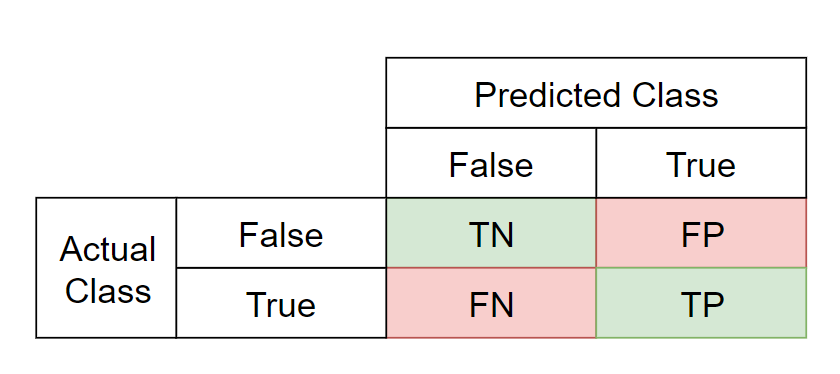
\includegraphics[scale = 0.4]{Images/2dconfusion.png}
        \caption{Confusion matrix for 2 classes.}
        \label{2classmatrix}
    \end{figure}
    
    Therefore, the most common metrics are: \\
    
    \begin{itemize}
        \item \textbf{Accuracy} (what \% of predictions were correct): $$ \cfrac{\text{number of corect predictions}}{\text{total number of predictions made}} = \cfrac{TP + TN}{TP + TN + FP + FN}$$ \\
        Probably the most straightforward and intuitive metric for classifier performance. However, it is misleading when confronted with class imbalance problem. \\
        
        \item \textbf{Precision} (what \% of positive predictions were correct): $$ \cfrac{TP}{TP + FP}$$ 
        In the context of fraud detection, it is usually more costly to miss a positive instance than to falsely label a negative instance. Hence, we are concerned with precision rather than recall. \\
        
        \item \textbf{Recall} (what \% of positive cases did model catch): $$ \cfrac{TP}{TP + FN}$$ \\
        In situations where you want to detect instances of a minority class, you are usually concerned more with recall than precision. \\
        
        \item \textbf{F1 score} (weighted average of precision and recall): $$ \cfrac{2(\text{precision} \ * \ \text{recall})}{\text{precision} \ + \ \text{recall}} = \cfrac{2TP}{2TP + FP + FN}$$ \\
        As all of the metrics above, F1 score takes values between 0 and 1, higher values indicating better performance. In fact, higher values of F1 score indicate better balance between precision and recall. \\ 
        
        \item \textbf{Matthew's Correlation Coefficient (MCC)} $$ \cfrac{TP * TN - FP * FN}{\sqrt{(TP + FP)(TP + FN)(TN + FP)(TN + FN)}}$$ \\
        Unlike the other metrics discussed above, MCC takes all the cells of the Confusion Matrix into consideration in its formula, hence behaves the best in case of imbalanced classes. The range of values of MCC lie between -1 to +1. A model with a score of +1 is a perfect model and -1 is a poor model, while a score of 0 is a as good as a random model. This property is one of the key usefulness of MCC as it leads to easy interpretability. \\
    \end{itemize}
    
    \subsubsection*{Metrics for MultiClass Classification}
    
    In order to extend the 2D confusion matrix for the general case, I will adopt a One-vs-All (OVA) classifiers approach which reduces the problem to binary classification. Specifically, each class will be in turn considered the positive/true class, while all the others merged will be the negative/false class. At each step, the metrics described in the previous subsection will be computed and afterwards combined in a couple of different ways to form their variations used for evaluating multiclass classification. \\
    
    \begin{figure}[H]
        \centering
        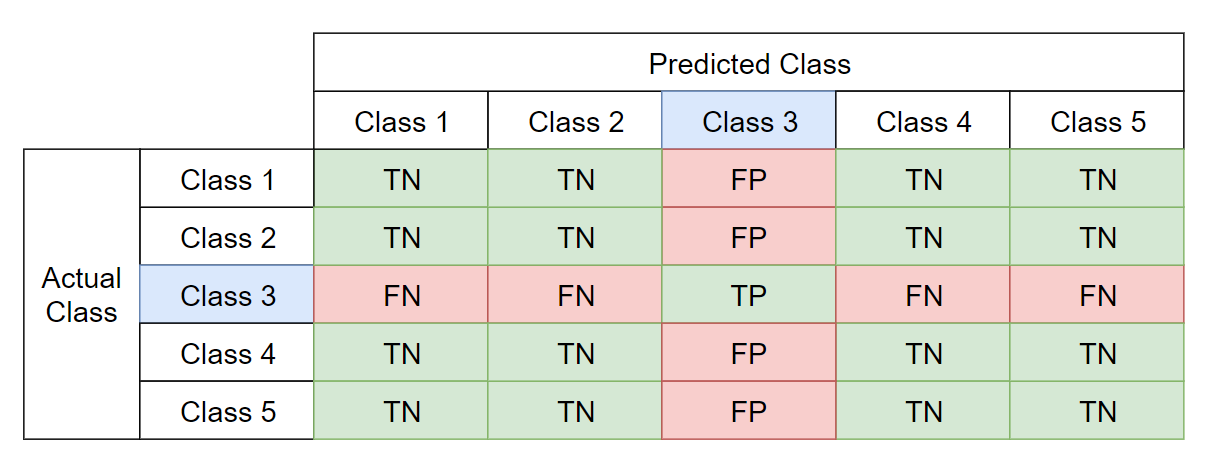
\includegraphics[scale = 0.5]{Images/5dconfusion.png}
        \caption{Confusion matrix for multiple classes using OVA approach where Class 3 is the positive class.}
        \label{5classmatrix}
    \end{figure}
    
    Let TP$_i$, TN$_i$, FP$_i$, FN$_i$ be the number of true positives, true negatives, false positives and false negatives when class $i$ is regarded as the positive class. Moreover, let Metric$_i$ be the value of an evaluation metric when class $i$ is regarded as the positive class, where Metric is one of Precision, Recall, F1 score, MCC (note that Accuracy will still be computed as before i.e. $ \frac{\text{number of corect predictions}}{\text{total number of predictions made}}$). Thus, Metric$_i$ is computed using TP$_i$, TN$_i$, FP$_i$, FN$_i$ as inputs. Given these definitions, there are two approaches to average the class specific metrics in order to obtain the metrics used for evaluating multiclass classifiers: \\
    
    \begin{itemize}
        \item \textbf{Micro Averaging}: \\
            Micro-Multiclass-Metric = Metric($\sum_{i=1}^{N}$ TP$_i$, $\sum_{i=1}^{N}$ TN$_i$, $\sum_{i=1}^{N}$ FP$_i$, $\sum_{i=1}^{N}$ FN$_i$) \\
             A micro-average will aggregate the contributions of all classes to compute the average metric. In a multi-class classification setup, micro-average is preferable when we suspect there might be class imbalance.
            
        \item \textbf{Macro Averaging}: \\
            Macro-Multiclass-Metric = $\cfrac{1}{N}$ $\sum_{i=1}^{N}$ Metric$_i$ \\
            A macro-average will compute the metric independently for each class and then take the average (hence treating all classes equally).
    \end{itemize}
    
    
    
    \subsection{Monte Carlo Permutation Test}
    
    In order to comparatively evaluate any two models implemented, I use the \textbf{permutation} \textbf{test}$^{\small \cite{permutation_test}}$ for paired samples. The permutation test checks whether the population mean of the two conditions is different (H$_1$) or the same (H$_0$). The power of the permutation test is defined as 1 - $\alpha$ where: 
    
    \begin{equation}
        \centering
        \alpha = \mathbb{P}(\text{Do not reject H$^0$ | H$_1$ is true}) \newline
    \end{equation}    
    i.e. the test declares no difference, where there really is one. \\
    
    I opted for the permutation test as it is known to have higher significance power than the, perhaps more popular, sign test$^{\small \cite{signtest}}$. The core assumption of the permutation test is that if the measured difference \textit{d} in mean M between systems A and B is an incident, i.e., if there is no real difference between them (because they come from one and the same distribution), it should not matter how many times one randomly swaps the two results. Consider \textit{n} paired results of System A and B. There are 2$^n$ ways of flipping or not flipping the n pairs of results, i.e., 2$^n$ permutations. These permutations operate row-wise. In other words, we create resamplings of these permutations in the following way: for each paired observation in the original runs, $a_i$ and $b_i$, a coin is flipped. If it comes up heads, then swap the score for $b_i$ with $a_i$. Otherwise, leave the pair unchanged. Now calculate the means M of the two system under this permutation, calculate their difference in means, and then do it 2$^n$ times for all permutations. Count how many of the 2$^n$ differences are as high as the difference in the unpermuted version. Call this number S. \\
    
    Finally, if due to a high number \textit{n}, the exponentially many resamplings computation is not feasible, then a large enough random subset of cardinality R should be tested. This version of the test is called \textbf{Monte Carlo Permutation Test}. The probability of observing the difference between the original runs by chance is approximated by: \\
    
    \begin{equation}
        p = \cfrac{S + 1}{R + 1}
    \end{equation}

    \smallskip
    
    I decide that two sets of predictions come from different distributions for p-value $\leq$ 0.05 and I choose R = 5000.
    
    \subsection{ML Pipeline Time and Space Performance Metrics}
    
    \section{Evaluation Results and Discussions} \label{Evaluation Results}

    \begin{figure}[H]
  \centering
  \centerline{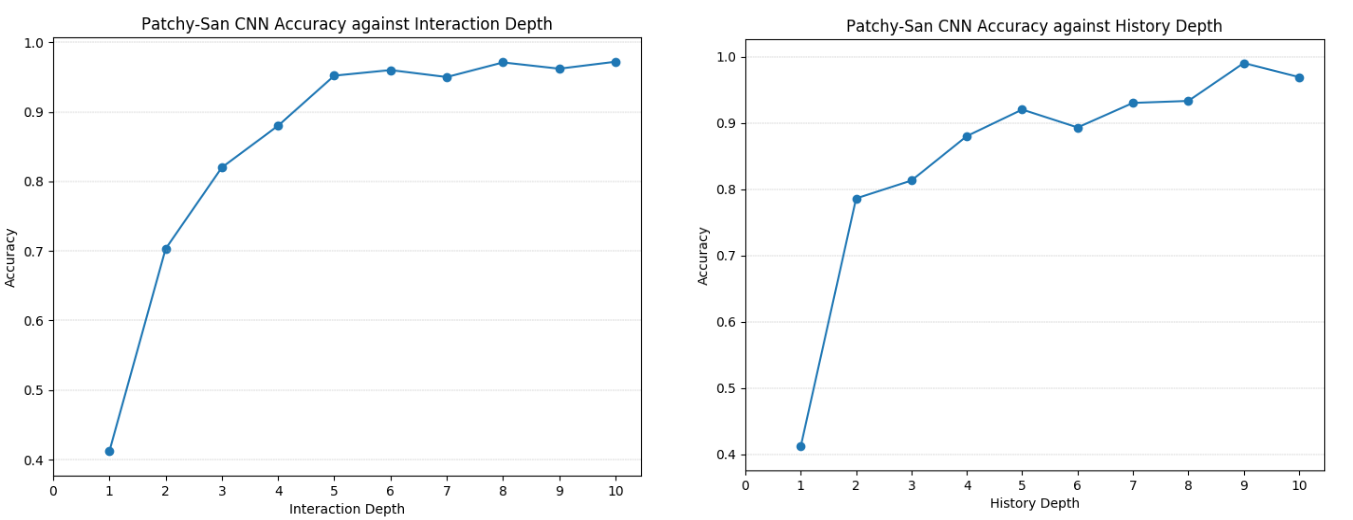
\includegraphics[scale=0.55]{Images/inter_hist_deph_acc.png}}
  \caption{ Figure showing accuracy scores for various values of $ID$ keeping $HD = 1$ (LHS) and 
            accuracy for various values of $HD$ keeping $ID = 1$ (RHS).}
  \label{inter_hist_depth_acc}
    \end{figure}
    
      \begin{figure}[H]
  \centering
  \centerline{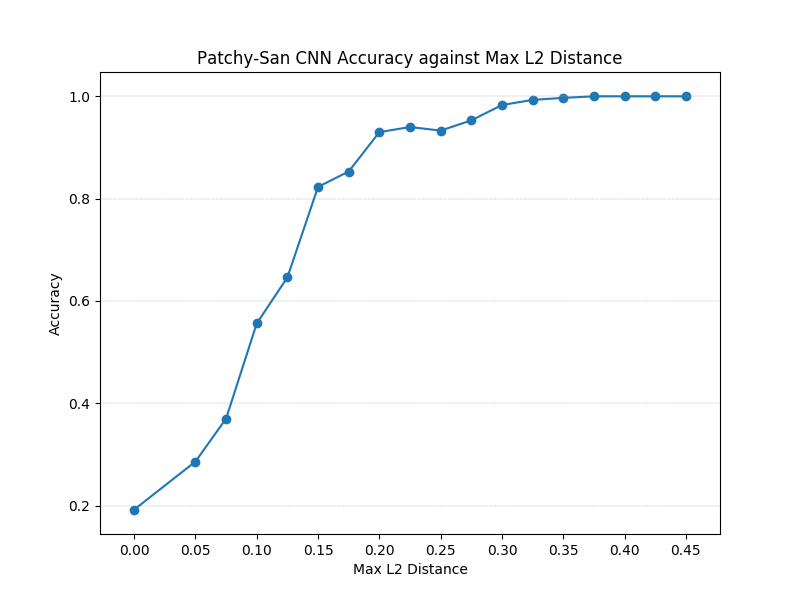
\includegraphics[scale=0.7]{Images/l2_dist.png}}
  \caption{ Figure showing accuracy scores for various values of maximum $L2_{distance}$ for $ID = 3$ and $HD = 4$.}
  \label{l2_dist}
    \end{figure}
    
    \begin{figure}[H]
  \centering
  \centerline{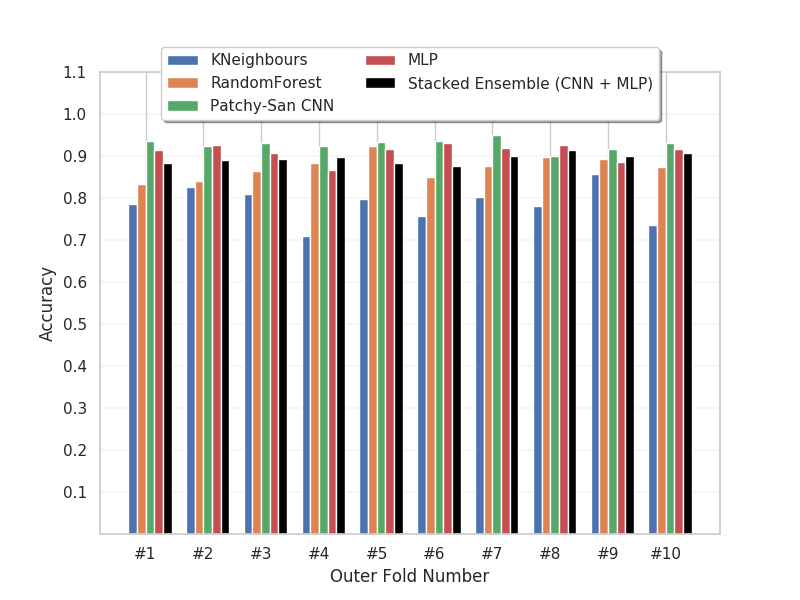
\includegraphics[scale=0.8]{Images/acc_per_fold_new_cols.png}}
  \caption{Comparative accuracy scores for all implemented models per outer fold.}
  \label{acc_per_fold}
\end{figure}

\begin{figure}[H]
  \centering
  \centerline{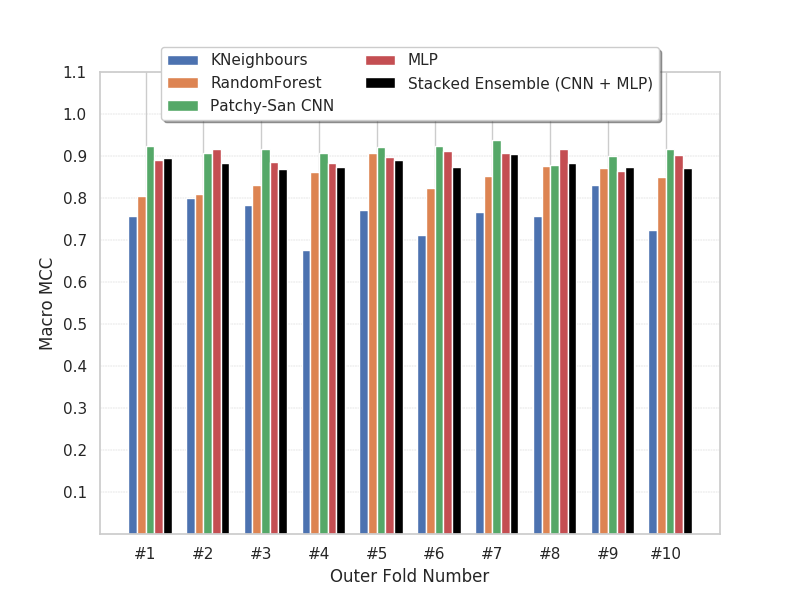
\includegraphics[scale=0.8]{Images/macro_mcc_per_fold_new_cols.png}}
  \caption{Comparative macro MCC scores for all implemented models per outer fold.}
  \label{macro_mcc_per_fold}
\end{figure}

\begin{figure}[H]
  \centering
  \centerline{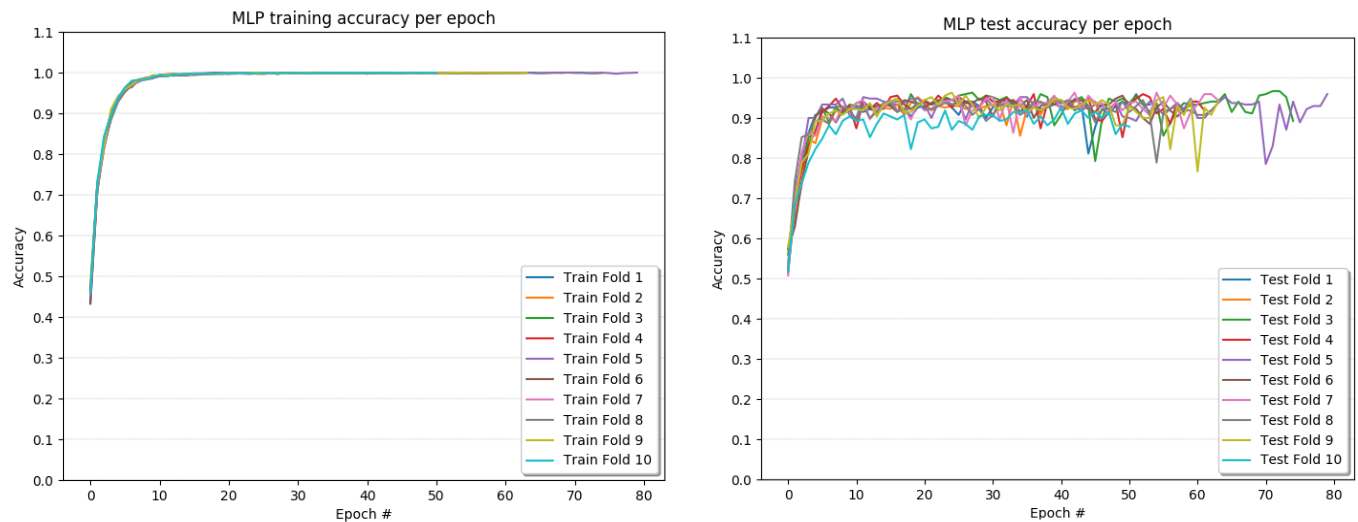
\includegraphics[scale=0.55]{Images/mlp_train_test.png}}
  \caption{MLP training and test accuracy against training epoch.}
  \label{cnn_train_test}
\end{figure}

\begin{figure}[H]
  \centering
  \centerline{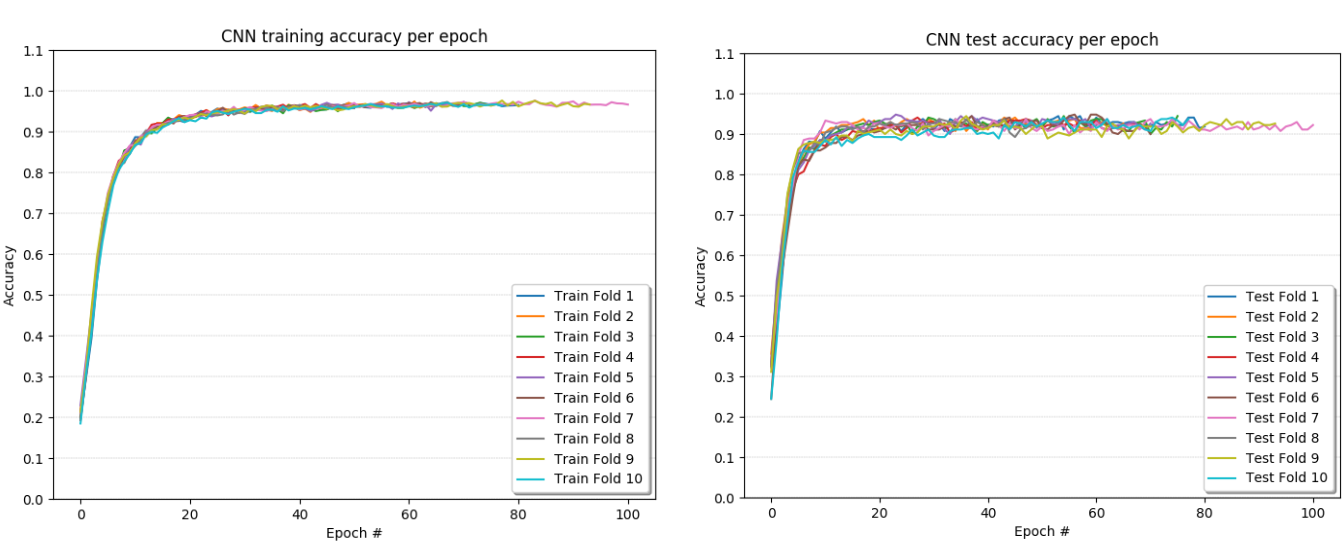
\includegraphics[scale=0.55]{Images/cnn_train_test.png}}
  \caption{CNN training and test accuracy against training epoch.}
  \label{mlp_train_test}
\end{figure}
\end{document}


